\section*{Introduction}
\hspace{\parindent}Pollution caused by the aircraft industry is a lot and this industry
has a lot of problems like aircraft noise which is considered one of
the main sources of noise pollution\cite{SakrRef} %here goes SalakawyRef[]
which directly has a lot of consequences and damages health
according to EASA, FAA, and other important international 
organizations, this made them set standards to the limit of 
noise caused by aircraft and drones, 
air pollution is also a very serious problem caused by the aircraft
and other vehicles that only plane traffic are responsible for 2\% of global energy-related $CO_2$ emission, %[unknown ref] 
this is a lot considering the number of flights, in addition, maintenance
of any mechanical part that has moving parts, complex design and
functionality is a major problem in aircraft so they may try to make
less moving parts or make them one part.\cite{SakrRef}

There is an application or engine that solves all the problems above no noise, no air pollution, no moving parts; this is ion propulsion aircraft
and it has a lot of uses and applications like micro drones, less than air aircraft, cooling systems, and most importantly are drones.\cite{SakrRef} Another common application of ion propulsion is space crafts and satellites, and NASA sees that ion propulsion is the key to deep space.\cite{NASARef}

A very common and basic system is ionocraft or lifer, generally, it consists of two electrodes one is sharp (wire in lifter example)
and the other is round (aluminum foil in the lifter example)
Fig.\ref{Lifter}, this makes an asymmetric capacitor and  under a high DC voltage, discharge happens (corona discharge) and this discharge ionizes the air around 
the electrodes
(ion wind), this wind produces a thrust that makes the lifter fly this is called Biefeld–Brown effect.\cite{first}, this seems simple but
providing an accurate model for this phenomenon was difficult and not fully understood\cite{aerodynamicModels}, we aim to seek and come up
with a good model for this phenomenon as it is the base-stone for all these applications.
\begin{figure}[ht]
	\centering
	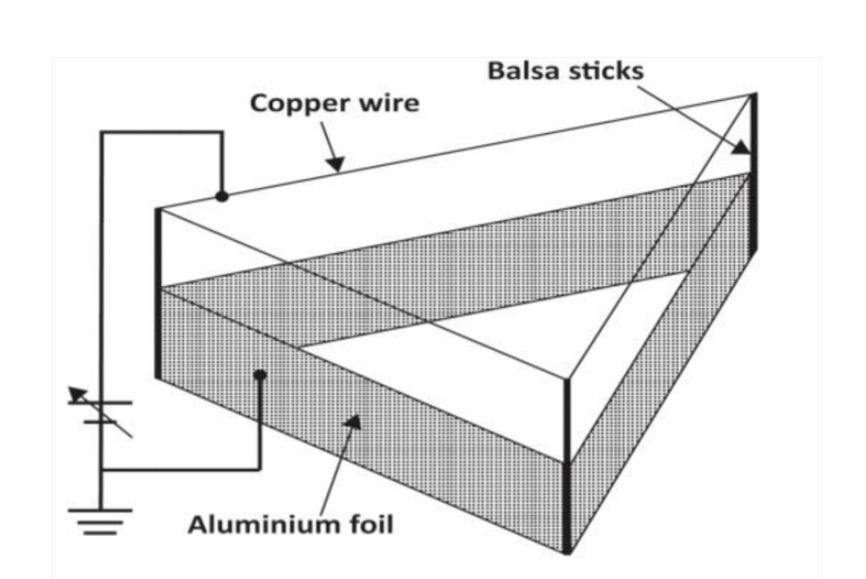
\includegraphics[scale=0.25]{images/Lifter.png}
  \caption{Lifter components\cite{first}}
	\label{Lifter}
\end{figure}
